% Options for packages loaded elsewhere
\PassOptionsToPackage{unicode}{hyperref}
\PassOptionsToPackage{hyphens}{url}
%
\documentclass[
  ignorenonframetext,
]{beamer}
\usepackage{pgfpages}
\setbeamertemplate{caption}[numbered]
\setbeamertemplate{caption label separator}{: }
\setbeamercolor{caption name}{fg=normal text.fg}
\beamertemplatenavigationsymbolsempty
% Prevent slide breaks in the middle of a paragraph
\widowpenalties 1 10000
\raggedbottom
\setbeamertemplate{part page}{
  \centering
  \begin{beamercolorbox}[sep=16pt,center]{part title}
    \usebeamerfont{part title}\insertpart\par
  \end{beamercolorbox}
}
\setbeamertemplate{section page}{
  \centering
  \begin{beamercolorbox}[sep=12pt,center]{part title}
    \usebeamerfont{section title}\insertsection\par
  \end{beamercolorbox}
}
\setbeamertemplate{subsection page}{
  \centering
  \begin{beamercolorbox}[sep=8pt,center]{part title}
    \usebeamerfont{subsection title}\insertsubsection\par
  \end{beamercolorbox}
}
\AtBeginPart{
  \frame{\partpage}
}
\AtBeginSection{
  \ifbibliography
  \else
    \frame{\sectionpage}
  \fi
}
\AtBeginSubsection{
  \frame{\subsectionpage}
}
\usepackage{lmodern}
\usepackage{amssymb,amsmath}
\usepackage{ifxetex,ifluatex}
\ifnum 0\ifxetex 1\fi\ifluatex 1\fi=0 % if pdftex
  \usepackage[T1]{fontenc}
  \usepackage[utf8]{inputenc}
  \usepackage{textcomp} % provide euro and other symbols
\else % if luatex or xetex
  \usepackage{unicode-math}
  \defaultfontfeatures{Scale=MatchLowercase}
  \defaultfontfeatures[\rmfamily]{Ligatures=TeX,Scale=1}
\fi
% Use upquote if available, for straight quotes in verbatim environments
\IfFileExists{upquote.sty}{\usepackage{upquote}}{}
\IfFileExists{microtype.sty}{% use microtype if available
  \usepackage[]{microtype}
  \UseMicrotypeSet[protrusion]{basicmath} % disable protrusion for tt fonts
}{}
\makeatletter
\@ifundefined{KOMAClassName}{% if non-KOMA class
  \IfFileExists{parskip.sty}{%
    \usepackage{parskip}
  }{% else
    \setlength{\parindent}{0pt}
    \setlength{\parskip}{6pt plus 2pt minus 1pt}}
}{% if KOMA class
  \KOMAoptions{parskip=half}}
\makeatother
\usepackage{xcolor}
\IfFileExists{xurl.sty}{\usepackage{xurl}}{} % add URL line breaks if available
\IfFileExists{bookmark.sty}{\usepackage{bookmark}}{\usepackage{hyperref}}
\hypersetup{
  pdftitle={Sampling Distributions, the Central Limit Theorem (CLT) and Confidence Intervals},
  pdfauthor={Sahir Rai Bhatnagar},
  hidelinks,
  pdfcreator={LaTeX via pandoc}}
\urlstyle{same} % disable monospaced font for URLs
\newif\ifbibliography
\usepackage{color}
\usepackage{fancyvrb}
\newcommand{\VerbBar}{|}
\newcommand{\VERB}{\Verb[commandchars=\\\{\}]}
\DefineVerbatimEnvironment{Highlighting}{Verbatim}{commandchars=\\\{\}}
% Add ',fontsize=\small' for more characters per line
\usepackage{framed}
\definecolor{shadecolor}{RGB}{248,248,248}
\newenvironment{Shaded}{\begin{snugshade}}{\end{snugshade}}
\newcommand{\AlertTok}[1]{\textcolor[rgb]{0.94,0.16,0.16}{#1}}
\newcommand{\AnnotationTok}[1]{\textcolor[rgb]{0.56,0.35,0.01}{\textbf{\textit{#1}}}}
\newcommand{\AttributeTok}[1]{\textcolor[rgb]{0.77,0.63,0.00}{#1}}
\newcommand{\BaseNTok}[1]{\textcolor[rgb]{0.00,0.00,0.81}{#1}}
\newcommand{\BuiltInTok}[1]{#1}
\newcommand{\CharTok}[1]{\textcolor[rgb]{0.31,0.60,0.02}{#1}}
\newcommand{\CommentTok}[1]{\textcolor[rgb]{0.56,0.35,0.01}{\textit{#1}}}
\newcommand{\CommentVarTok}[1]{\textcolor[rgb]{0.56,0.35,0.01}{\textbf{\textit{#1}}}}
\newcommand{\ConstantTok}[1]{\textcolor[rgb]{0.00,0.00,0.00}{#1}}
\newcommand{\ControlFlowTok}[1]{\textcolor[rgb]{0.13,0.29,0.53}{\textbf{#1}}}
\newcommand{\DataTypeTok}[1]{\textcolor[rgb]{0.13,0.29,0.53}{#1}}
\newcommand{\DecValTok}[1]{\textcolor[rgb]{0.00,0.00,0.81}{#1}}
\newcommand{\DocumentationTok}[1]{\textcolor[rgb]{0.56,0.35,0.01}{\textbf{\textit{#1}}}}
\newcommand{\ErrorTok}[1]{\textcolor[rgb]{0.64,0.00,0.00}{\textbf{#1}}}
\newcommand{\ExtensionTok}[1]{#1}
\newcommand{\FloatTok}[1]{\textcolor[rgb]{0.00,0.00,0.81}{#1}}
\newcommand{\FunctionTok}[1]{\textcolor[rgb]{0.00,0.00,0.00}{#1}}
\newcommand{\ImportTok}[1]{#1}
\newcommand{\InformationTok}[1]{\textcolor[rgb]{0.56,0.35,0.01}{\textbf{\textit{#1}}}}
\newcommand{\KeywordTok}[1]{\textcolor[rgb]{0.13,0.29,0.53}{\textbf{#1}}}
\newcommand{\NormalTok}[1]{#1}
\newcommand{\OperatorTok}[1]{\textcolor[rgb]{0.81,0.36,0.00}{\textbf{#1}}}
\newcommand{\OtherTok}[1]{\textcolor[rgb]{0.56,0.35,0.01}{#1}}
\newcommand{\PreprocessorTok}[1]{\textcolor[rgb]{0.56,0.35,0.01}{\textit{#1}}}
\newcommand{\RegionMarkerTok}[1]{#1}
\newcommand{\SpecialCharTok}[1]{\textcolor[rgb]{0.00,0.00,0.00}{#1}}
\newcommand{\SpecialStringTok}[1]{\textcolor[rgb]{0.31,0.60,0.02}{#1}}
\newcommand{\StringTok}[1]{\textcolor[rgb]{0.31,0.60,0.02}{#1}}
\newcommand{\VariableTok}[1]{\textcolor[rgb]{0.00,0.00,0.00}{#1}}
\newcommand{\VerbatimStringTok}[1]{\textcolor[rgb]{0.31,0.60,0.02}{#1}}
\newcommand{\WarningTok}[1]{\textcolor[rgb]{0.56,0.35,0.01}{\textbf{\textit{#1}}}}
\usepackage{longtable,booktabs}
\usepackage{caption}
% Make caption package work with longtable
\makeatletter
\def\fnum@table{\tablename~\thetable}
\makeatother
\usepackage{graphicx,grffile}
\makeatletter
\def\maxwidth{\ifdim\Gin@nat@width>\linewidth\linewidth\else\Gin@nat@width\fi}
\def\maxheight{\ifdim\Gin@nat@height>\textheight\textheight\else\Gin@nat@height\fi}
\makeatother
% Scale images if necessary, so that they will not overflow the page
% margins by default, and it is still possible to overwrite the defaults
% using explicit options in \includegraphics[width, height, ...]{}
\setkeys{Gin}{width=\maxwidth,height=\maxheight,keepaspectratio}
% Set default figure placement to htbp
\makeatletter
\def\fps@figure{htbp}
\makeatother
\setlength{\emergencystretch}{3em} % prevent overfull lines
\providecommand{\tightlist}{%
  \setlength{\itemsep}{0pt}\setlength{\parskip}{0pt}}
\setcounter{secnumdepth}{-\maxdimen} % remove section numbering
\usepackage{default}
\usepackage{animate} %need the animate.sty file 
\usepackage{graphicx}
%\graphicspath{{/home/sahir/Dropbox/jobs/laval/minicours/slides/}}
\usepackage{hyperref, url}
%\usepackage[round,sort]{natbib}   % bibliography omit 'round' option if you prefer square brackets
%\bibliographystyle{apalike}
\usepackage{biblatex}
\bibliography{bib.bib}
% Removes icon in bibliography
\setbeamertemplate{bibliography item}[text]

\usepackage[normalem]{ulem}

\setbeamertemplate{theorems}[numbered]

\setbeamertemplate{caption}[numbered]
\setbeamertemplate{caption label separator}{: }
\setbeamercolor{caption name}{fg=normal text.fg}

%\newtheorem{prop}{Proposition}
%\newenvironment{theoremc}[1]
%{\begin{shaded}\begin{theorem}[#1]}
%		{\end{theorem}\end{shaded}}

%\newtheorem{examplefirst}{Example}
%\newtheorem{examplesecond}{Example}
%\newenvironment<>{examplefirst}[1][]{%
%	\setbeamercolor{block title example}{bg=lightgray}%
%	\begin{example}#2[#1]}{\end{example}}
%\newenvironment<>{examplesecond}[1][]{%
%	\setbeamercolor{block title example}{fg=white,bg=blue!75!black}%
%	\begin{example}#2[#1]}{\end{example}}	

%\usepackage{amsthm}


\usepackage[figurename=Fig.]{caption}
\usepackage{subfig}
\usepackage{tikz, pgfplots,epsfig}
\usetikzlibrary{arrows,shapes.geometric}
\usepackage{color, colortbl,xcolor}
\definecolor{lightgray}{RGB}{200,200,200}
\definecolor{palegray}{RGB}{221,221,221}
\definecolor{myblue}{RGB}{0,89,179}
\definecolor{myorange}{rgb}{0.776,0.357,0.157}
\usepackage{comment}
\setbeamercolor{frametitle}{fg=myblue}
\setbeamercolor{section in head/foot}{bg=myblue, fg=white}
\setbeamercolor{author in head/foot}{bg=myblue}
\setbeamercolor{date in head/foot}{bg=myblue}

\usepackage{shadethm}
%\colorlet{shadecolor}{blue!15}
\colorlet{shadecolor}{palegray}
%\setlength{\shadeboxrule}{.4pt}

\newshadetheorem{thm}{Theorem}
\newshadetheorem{defm}{Definition}
\newshadetheorem{exm}{Exercise}
\newshadetheorem{remarkm}{Remark}
%\definecolor{shadethmcolor}{HTML}{EDF8FF}
\definecolor{shadethmcolor}{RGB}{221,221,221}
%\definecolor{shaderulecolor}{HTML}{45CFFF}
\definecolor{shaderulecolor}{RGB}{0,89,179}
\setlength{\shadeboxrule}{.4pt}


\usepackage{array}
\newcolumntype{L}{>{\centering\arraybackslash}m{3cm}} % used for text wrapping in ctable
\usepackage{ctable}
\usepackage[utf8]{inputenc}
\usepackage{fontenc}
\usepackage{pifont}% http://ctan.org/pkg/pifont
\newcommand{\cmark}{\ding{51}}%
\newcommand{\xmark}{\ding{55}}%
\def\widebar#1{\overline{#1}}
\definecolor{whitesmoke}{rgb}{0.96, 0.96, 0.96}

\usepackage{amssymb}
\usepackage{amsmath}

\usepackage{bm}
\def\transpose{{\sf{T}}}
\def\E{{\skew0\bm{E}}}
\def\Xvec{{\skew0\bm{X}}}
\def\Xveca{{\skew0\bm{X}}_1}
\def\Xvecb{{\skew0\bm{X}}_2}

\def\Yvec{{\skew0\bm{Y}}}
\def\bmY{{\skew0\bm{Y}}}
\def\bmX{{\skew0\bm{X}}}
\def\bmy{{\skew0\bm{y}}}
\def\bmG{{\skew0\bm{G}}}
\def\bmS{{\skew0\bm{S}}}
\def\bmA{{\skew0\bm{A}}}
\def\bmB{{\skew0\bm{B}}}
\def\bmD{{\skew0\bm{D}}}
\def\bmI{{\skew0\bm{I}}}
\def\bmV{{\skew0\bm{V}}}
\def\bmU{{\skew0\bm{U}}}
\def\bv{{\skew0\bm{v}}}
\def\bw{{\skew0\bm{w}}}
\def\bmm{{\skew0\bm{m}}}
\def\bmzero{{\skew0\bm{0}}}
\def\bx{{\skew0\bm{x}}}
\def\xveca{{\skew0\bm{x}}_1}
\def\xvecb{{\skew0\bm{x}}_2}

\def\N{{\skew0\mathcal{N}}}
\def\T{{\small T}}

\def\mvec{{\skew0\bm{m}}}
\def\bmmu{{\skew0\bm{\mu}}}
\def\muvec{{\skew0\bm{\mu}}}
\def\balpha{{\skew0\bm{\alpha}}}
\def\bbeta{{\skew0\bm{\beta}}}
\def\bmtheta{{\skew0\bm{\theta}}}
\def\btheta{{\skew0\bm{\theta}}}

\def\cvec{{\skew0\mathbf{c}}}

\def\Xbar{\overline{X}}

\definecolor{lightgray}{rgb}{0.91,0.91,0.91}
\definecolor{purpleblue}{rgb}{0.50,0.50,1.00}

\pgfplotsset{compat=1.16}



\usepackage{fontspec}
%\setsansfont{Fira Sans}
%\setmonofont{Fira Mono}
%\setsansfont[ItalicFont={Fira Sans Light Italic},BoldFont={Fira Sans},BoldItalicFont={Fira Sans Italic}]{Fira Sans Light}
%\setmonofont[BoldFont={Fira Mono Medium}]{Fira Mono}

\def\installpath{/usr/local/share/texmf/fonts/opentype/libertinus/}
\setmainfont{LibertinusSerif}[
UprightFont    = *-Regular,
BoldFont       = *-Bold,
ItalicFont     = *-Italic,
BoldItalicFont = *-BoldItalic,
Ligatures      = TeX,
Extension      = .otf,
Path           = \installpath/
]

\setsansfont{LibertinusSerif}[
UprightFont    = *-Regular,
BoldFont       = *-Bold,
ItalicFont     = *-Italic,
BoldItalicFont = *-BoldItalic,
Ligatures      = TeX,
Extension      = .otf,
Path           = \installpath/
]


\setmonofont{LibertinusSerif}[
UprightFont    = *-Regular,
BoldFont       = *-Bold,
ItalicFont     = *-Italic,
BoldItalicFont = *-BoldItalic,
Ligatures      = TeX,
Extension      = .otf,
Path           = \installpath/
]



\setbeamercolor{itemize item}{fg=myblue}
%\setbeamertemplate{itemize item}[square]
\setbeamertemplate{itemize items}[circle]
\setbeamertemplate{blocks}[rounded][shadow=true]


%\setbeamertemplate{navigation symbols}{\usebeamercolor[fg]{title in head/foot}\usebeamerfont{title in head/foot}\insertframenumber}


%\setbeamertemplate{footline}{}

\beamertemplatenavigationsymbolsempty % toggle off if you want navigation symbols at the bottom

\setbeamertemplate{footline}
{ \usebeamercolor[fg]{page number in head/foot}%
	\usebeamerfont{page number in head/foot}%
	\hspace{1em}\insertsectionhead%
	\hfill%
	\insertframenumber\,/\,\hyperlinkappendixstart{\insertmainframenumber}
	\ifnum \thepage = \insertframeendpage{\small .}\else{\phantom{\small .}}\fi
	\hspace{1em}
	\vskip2pt%
}

\newtheorem{proposition}[theorem]{Proposition}
\newtheorem{exercise}[theorem]{Exercise}

\titlegraphic{\hfill
\includegraphics[height=1cm]{../mcgill_logo.png}}


%% You also use hyperref, and pick colors 
\hypersetup{colorlinks,citecolor=myorange,filecolor=red,linkcolor=brown,urlcolor=blue}

\newcommand {\framedgraphiccaption}[2] {
	\begin{figure}
		\centering
		\includegraphics[width=\textwidth,height=0.8\textheight,keepaspectratio]{#1}
		\caption{#2}
	\end{figure}
}

\newcommand {\framedgraphic}[1] {
	\begin{figure}
		\centering
		\includegraphics[width=\textwidth,height=0.9\textheight,keepaspectratio]{#1}
	\end{figure}
}


\AtBeginSection[]{
	\begin{frame}
		\vfill
		\centering
		\begin{beamercolorbox}[sep=8pt,center,shadow=true,rounded=true]{title}
			\usebeamerfont{title}\insertsectionhead\par%
		\end{beamercolorbox}
		\vfill
	\end{frame}
}

\newcommand\Wider[2][3em]{%
	\makebox[\linewidth][c]{%
		\begin{minipage}{\dimexpr\textwidth+#1\relax}
			\raggedright#2
		\end{minipage}%
	}%
}


\makeatletter

\def \iqsssectiontitleheader {}

\newcommand{\iqsssectiontitle}[1]{
	\def \iqsssectiontitleheader{#1}
}

\@ifundefined{insertmainframenumber}
{%
	% \insertmainframenumber not defined
	\newcommand{\insertmainframenumber}{\inserttotalframenumber}
}
{%
	% \insertmainframenumber already defined
}%


\AtBeginSection[]{
	\title{\insertsectionhead}
	{
		%\definecolor{white}{RGB}{140,193,250}
		%\definecolor{white}{RGB}{200,200,200}
		%\definecolor{white}{RGB}{242,244,247}
		\definecolor{white}{RGB}{0,89,179}
		%\definecolor{iqss@orange}{rgb}{1,1,1}
		\ifnum \insertmainframenumber > \insertframenumber
		%\setbeamercolor{background canvas}{bg=myblue}
		%\setbeamercolor{normal text}{fg=black,bg=white}
		%\setbeamercolor{frametitle}{fg=red}
		%\setbeamercolor{section in toc}{fg=myblue, bg=white}
		%\setbeamercolor{subsection in toc}{fg=myblue, bg=white}
		\frame{
			\frametitle{\iqsssectiontitleheader}
			\tableofcontents[currentsection]
		}
		\else
		\frame{
			\frametitle{Backup Slides}
			\tableofcontents[sectionstyle=shaded/shaded,subsectionstyle=shaded/shaded/shaded]
		}
		\fi
	}
}
\makeatother

\title{Sampling Distributions, the Central Limit Theorem (CLT) and Confidence
Intervals}
\author{Sahir Rai Bhatnagar}
\date{Last compiled on August 30, 2020}
\institute{EPIB 607\newline Department of Epidemiology, Biostatistics, and
Occupational Health \newline McGill University\newline}

\begin{document}
\frame{\titlepage}

\hypertarget{data-basics}{%
\section{Data basics}\label{data-basics}}

\begin{frame}[fragile]{Hello}
\protect\hypertarget{hello}{}

\scriptsize

\begin{Shaded}
\begin{Highlighting}[]
\KeywordTok{plot}\NormalTok{(}\KeywordTok{rnorm}\NormalTok{(}\DecValTok{10}\NormalTok{))}
\end{Highlighting}
\end{Shaded}

\begin{center}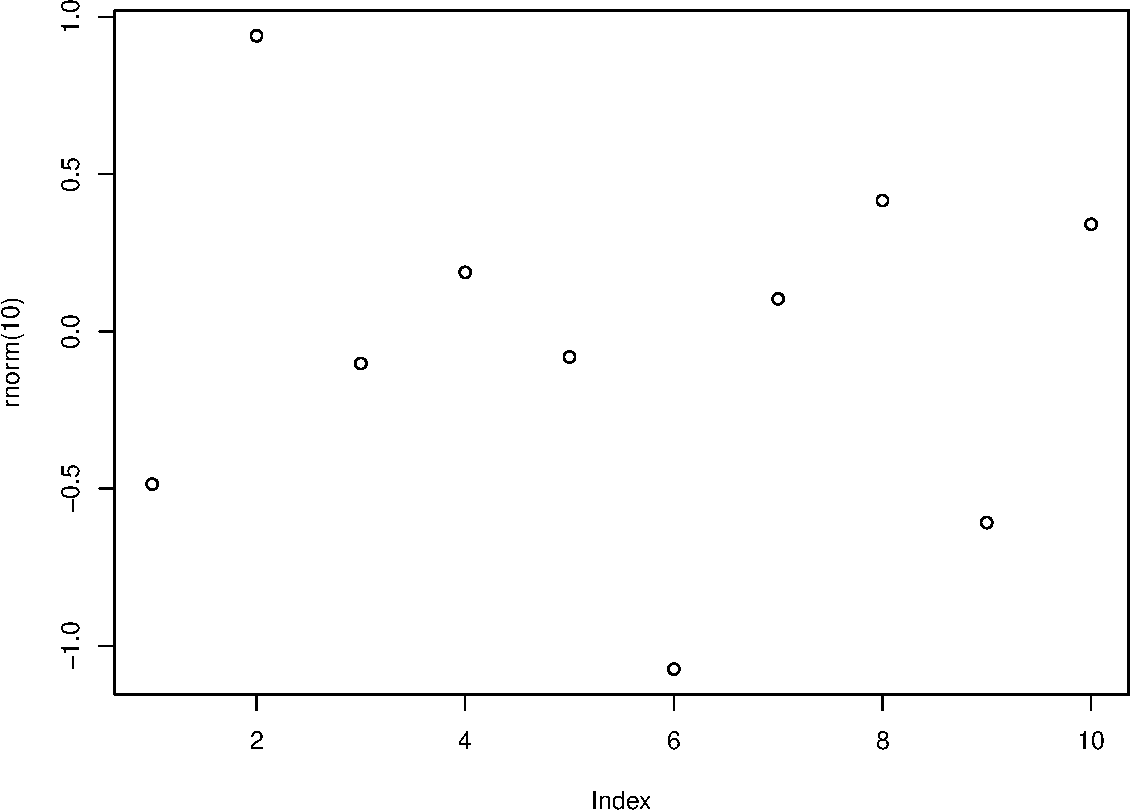
\includegraphics[width=1\linewidth]{001-exploring-data_files/figure-beamer/testing-1} \end{center}

\normalsize

\end{frame}

\begin{frame}[fragile]{Example: Iowa vs.~Illinois}
\protect\hypertarget{example-iowa-vs.-illinois}{}

\scriptsize

\begin{Shaded}
\begin{Highlighting}[]
\KeywordTok{library}\NormalTok{(covdata)}
\KeywordTok{library}\NormalTok{(dplyr)}
\KeywordTok{library}\NormalTok{(ggplot2)}
\CommentTok{# library(tidyverse)}
\end{Highlighting}
\end{Shaded}

\normalsize

\scriptsize

\begin{Shaded}
\begin{Highlighting}[]
\CommentTok{# drat::addRepo("kjhealy")}
\CommentTok{# install.packages("covdata")}

\CommentTok{# unique(nytcovcounty$state)}
\CommentTok{# dim(nytcovcounty)}

\NormalTok{county_pop <-}\StringTok{ }\KeywordTok{read.csv}\NormalTok{(}\StringTok{"https://raw.githubusercontent.com/simonw/covid-19-datasette/master/us_census_county_populations_2019.csv"}\NormalTok{)}
\KeywordTok{data}\NormalTok{(}\StringTok{"nytcovcounty"}\NormalTok{)}
\CommentTok{# county_pop}

\NormalTok{p1 <-}\StringTok{ }\NormalTok{nytcovcounty }\OperatorTok
\StringTok{  }\NormalTok{dplyr}\OperatorTok{::}\KeywordTok{filter}\NormalTok{(state }\OperatorTok\StringTok{ }\KeywordTok{c}\NormalTok{(}\StringTok{"Iowa"}\NormalTok{,}\StringTok{"Illinois"}\NormalTok{)) }\OperatorTok\StringTok{ }
\StringTok{  }\KeywordTok{mutate}\NormalTok{(}\DataTypeTok{uniq_name =} \KeywordTok{paste}\NormalTok{(county, state)) }\OperatorTok\StringTok{ }\CommentTok{# Can't use FIPS because of how the NYT bundled cities}
\StringTok{  }\KeywordTok{group_by}\NormalTok{(uniq_name) }\OperatorTok
\StringTok{  }\KeywordTok{mutate}\NormalTok{(}\DataTypeTok{days_elapsed =}\NormalTok{ date }\OperatorTok{-}\StringTok{ }\KeywordTok{min}\NormalTok{(date)) }\OperatorTok
\StringTok{  }\KeywordTok{ggplot}\NormalTok{(}\KeywordTok{aes}\NormalTok{(}\DataTypeTok{x =}\NormalTok{ days_elapsed, }\DataTypeTok{y =}\NormalTok{ cases, }\DataTypeTok{group =}\NormalTok{ uniq_name)) }\OperatorTok{+}\StringTok{ }
\StringTok{  }\KeywordTok{geom_line}\NormalTok{(}\DataTypeTok{size =} \FloatTok{0.25}\NormalTok{, }\DataTypeTok{color =} \StringTok{"gray20"}\NormalTok{) }\OperatorTok{+}\StringTok{ }
\StringTok{  }\KeywordTok{scale_y_log10}\NormalTok{(}\DataTypeTok{labels =}\NormalTok{ scales}\OperatorTok{::}\KeywordTok{label_number_si}\NormalTok{()) }\OperatorTok{+}\StringTok{ }
\StringTok{  }\KeywordTok{guides}\NormalTok{(}\DataTypeTok{color =} \OtherTok{FALSE}\NormalTok{) }\OperatorTok{+}\StringTok{ }
\StringTok{  }\KeywordTok{facet_wrap}\NormalTok{(}\OperatorTok{~}\StringTok{ }\NormalTok{state, }\DataTypeTok{ncol =} \DecValTok{5}\NormalTok{) }\OperatorTok{+}\StringTok{ }
\StringTok{  }\KeywordTok{labs}\NormalTok{(}\DataTypeTok{title =} \StringTok{"COVID-19 Cumulative Recorded Cases by US County"}\NormalTok{,}
       \DataTypeTok{subtitle =} \KeywordTok{paste}\NormalTok{(}\StringTok{"New York is bundled into a single area in this data.}\CharTok{\textbackslash{}n}\StringTok{Data as of"}\NormalTok{, }\KeywordTok{format}\NormalTok{(}\KeywordTok{max}\NormalTok{(nytcovcounty}\OperatorTok{$}\NormalTok{date), }\StringTok{"%A, %B %e, %Y"}\NormalTok{)),}
       \DataTypeTok{x =} \StringTok{"Days since first case"}\NormalTok{, }\DataTypeTok{y =} \StringTok{"Count of Cases (log 10 scale)"}\NormalTok{, }
       \DataTypeTok{caption =} \StringTok{"Data: The New York Times | Graph: @kjhealy"}\NormalTok{) }\OperatorTok{+}\StringTok{ }
\StringTok{  }\KeywordTok{theme_minimal}\NormalTok{()}

\NormalTok{p1}
\end{Highlighting}
\end{Shaded}

\begin{center}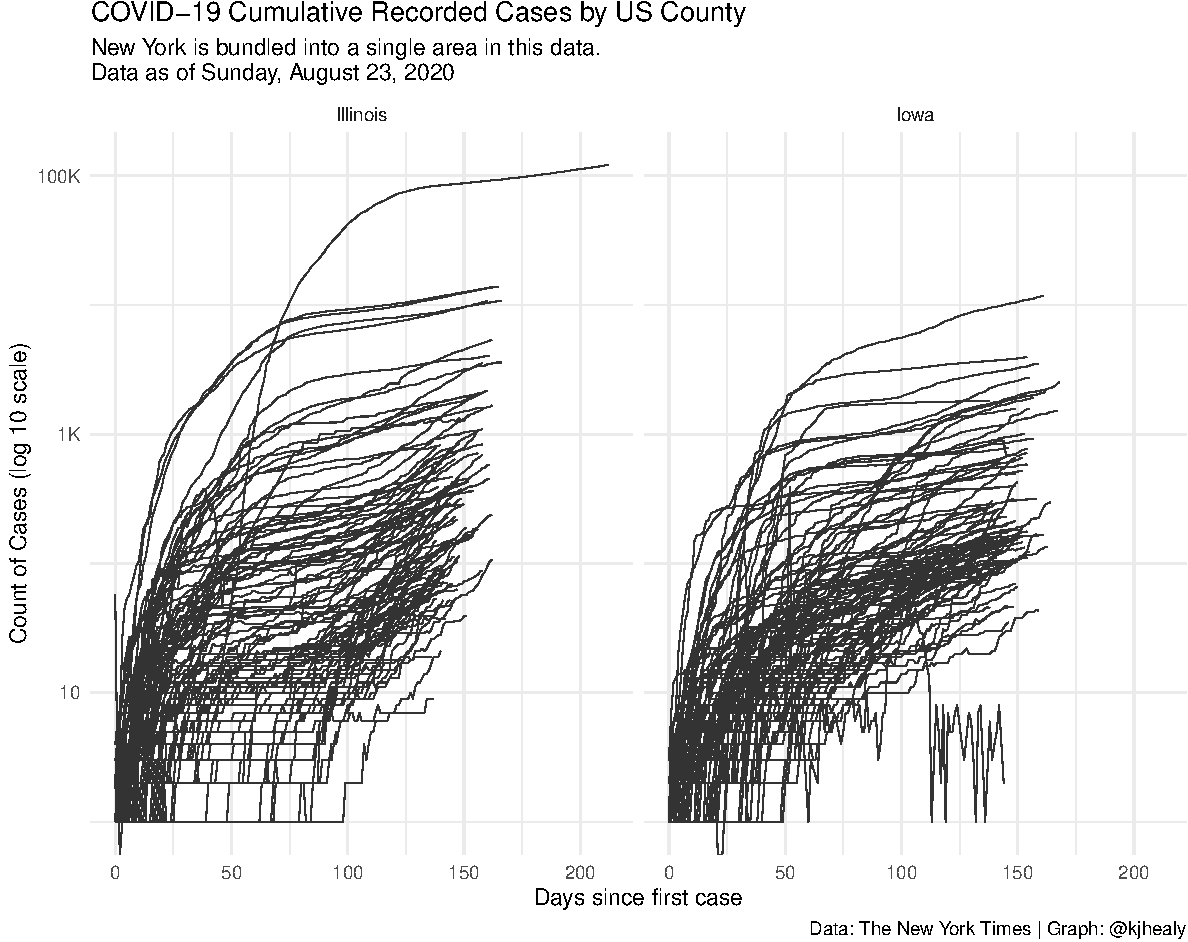
\includegraphics[width=1\linewidth]{001-exploring-data_files/figure-beamer/unnamed-chunk-2-1} \end{center}

\normalsize

\end{frame}

\begin{frame}{Example: the \emph{FAMuSS} study}
\protect\hypertarget{example-the-famuss-study}{}

\emph{The Functional SNPs Associated with Muscle Size and Strength}
(FAMuSS) study and data is introduced in \emph{OI Biostat}, Section
1.2.2.

One goal of the study---examine the association of demographic,
physiological and genetic characteristics with muscle strength.

\begin{itemize}
\tightlist
\item
  In simpler terms, study the ``sports gene'' \emph{ACTN3}.
\end{itemize}

\end{frame}

\begin{frame}{Four rows from \emph{FAMuSS} data matrix}
\protect\hypertarget{four-rows-from-famuss-data-matrix}{}

\captionsetup[table]{labelformat=empty}

\scriptsize

\normalsize

\scriptsize

\begin{longtable}[]{@{}lrlrrlr@{}}
\caption{\emph{OI Biostat} Table 1.6}\tabularnewline
\toprule
sex & age & race & height & weight & actn3.r577x &
ndrm.ch\tabularnewline
\midrule
\endfirsthead
\toprule
sex & age & race & height & weight & actn3.r577x &
ndrm.ch\tabularnewline
\midrule
\endhead
Female & 27 & Caucasian & 65.0 & 199 & CC & 40.0\tabularnewline
Male & 36 & Caucasian & 71.7 & 189 & CT & 25.0\tabularnewline
Female & 24 & Caucasian & 65.0 & 134 & CT & 40.0\tabularnewline
Female & 30 & Caucasian & 64.0 & 134 & CC & 43.8\tabularnewline
\bottomrule
\end{longtable}

\normalsize

\end{frame}

\begin{frame}{\emph{FAMuSS} Variables and their descriptions}
\protect\hypertarget{famuss-variables-and-their-descriptions}{}

\begin{center}
    \begin{tabular}{ll}
        {\bf Variable} & {\bf Description} \\
        & \\
        \texttt{sex} & Sex of the participant \\
        \texttt{age} & Age in years   \\
        \texttt{race} & Recorded as African Am (African American),\\
           & Caucasian, Asian, Hispanic, Other \\
        \texttt{height} & Height in inches    \\
        \texttt{weight} & Weight in pounds  \\
        \texttt{actn3.r577x} & Genotype at the location r577x in the ACTN3 gene. \\
        \texttt{ndrm.ch} & Percent change in strength in the non-dominant arm, \\
          & comparing strength after to before training \\
    \end{tabular}
\end{center}

\end{frame}

\begin{frame}{Types of Variables}
\protect\hypertarget{types-of-variables}{}

\textbf{Numerical variables} take on numerical values, such that
numerical operations (sums, differences, etc.) are reasonable.

\begin{itemize}
\item
  Discrete: only take on integer values (e.g., \# of family members)
\item
  Continuous: can take on any value within a specified range (e.g.,
  height)
\end{itemize}

\textbf{Categorical variables} take on values that are names or labels;
the possible values are called the variable's \emph{levels}.

\begin{itemize}
\tightlist
\item
  Ordinal: exists some natural ordering of levels (e.g., education)
\item
  Nominal: no natural ordering of levels (e.g., gender)
\end{itemize}

\end{frame}

\begin{frame}{Types of variables}
\protect\hypertarget{types-of-variables-1}{}

\begin{figure}
\centering
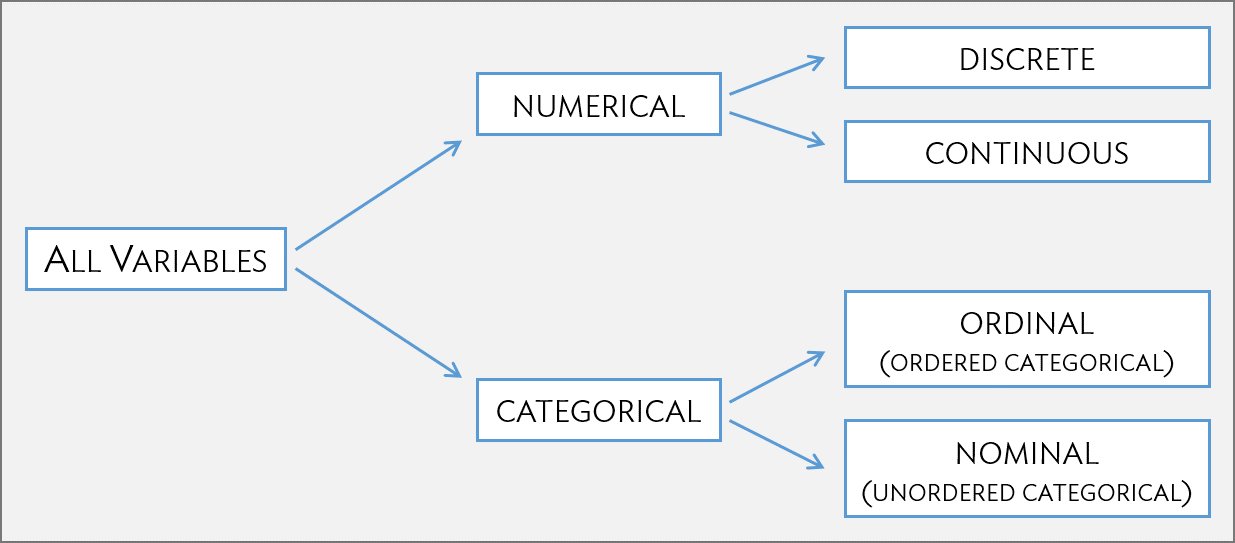
\includegraphics{figures/variableTypes.png}
\caption{alt data\_types}
\end{figure}

\end{frame}

\begin{frame}{Exploring data with simple tools}
\protect\hypertarget{exploring-data-with-simple-tools}{}

Techniques for exploring and summarizing data differ for numerical
versus categorical variables.

Numerical and graphical summaries are useful for examining variables one
at a time, but also for exploring the relationships between variables.

\end{frame}

\hypertarget{numerical-data}{%
\section{Numerical data}\label{numerical-data}}

\begin{frame}{Distributions and summary measures}
\protect\hypertarget{distributions-and-summary-measures}{}

The collection of values for a numerical, continuous variable (e.g.,
\texttt{weight}) is the \emph{distribution} for that variable.

Numerical and graphical summaries convey characteristics of a
distribution without listing all the values.

Important characteristics include\ldots{}

\begin{itemize}
\tightlist
\item
  Center: where is the middle of the distribution?

  \begin{itemize}
  \tightlist
  \item
    Measures of center: mean, median
  \end{itemize}
\item
  Spread: how similar or varied are the values to each other?

  \begin{itemize}
  \tightlist
  \item
    Measures of spread: standard deviation, interquartile range
  \end{itemize}
\end{itemize}

\end{frame}

\begin{frame}[fragile]{Measures of center}
\protect\hypertarget{measures-of-center}{}

The \emph{sample mean} of a variable is the sum of all observations
divided by the number of observations:

\[\overline{x} = \frac{x_1+x_2+\cdots+x_n}{n}\]\\
where \(x_1, x_2, \ldots, x_n\) represent the \(n\) observed values in a
sample.

The mean weight in \texttt{famuss} is 155.65 pounds:

\scriptsize

\begin{Shaded}
\begin{Highlighting}[]
\KeywordTok{mean}\NormalTok{(famuss}\OperatorTok{$}\NormalTok{weight)}
\end{Highlighting}
\end{Shaded}

\begin{verbatim}
## [1] 155.6479
\end{verbatim}

\normalsize

\end{frame}

\begin{frame}[fragile]{Measures of center \ldots{}}
\protect\hypertarget{measures-of-center-1}{}

The \emph{median} is the value of the middle observation in a sample.

If the number of observations is

\begin{itemize}
\tightlist
\item
  Odd, the median is the middle observation
\item
  Even, the median is the average of the two middle observations
\end{itemize}

The median is the \(50^{th}\) percentile; 50\% of observations lie
below/above the median.

\scriptsize

\begin{Shaded}
\begin{Highlighting}[]
\KeywordTok{median}\NormalTok{(famuss}\OperatorTok{$}\NormalTok{weight)}
\end{Highlighting}
\end{Shaded}

\begin{verbatim}
## [1] 150
\end{verbatim}

\normalsize

\end{frame}

\begin{frame}{Measures of spread}
\protect\hypertarget{measures-of-spread}{}

The \emph{standard deviation} measures (approximately) the distance
between a typical observation and the mean.

\begin{itemize}
\item
  An observation's \emph{deviation} is the distance between its value
  \(x\) and the sample mean \(\overline{x}\): \(x - \overline{x}\).
\item
  The \emph{sample variance} \(s^2\) is the sum of squared deviations
  divided by the number of observations minus 1.
  \[s^2 = \frac{({x_1 - \overline{x})}^{2}+({x_2 - \overline{x})}^{2}+\cdots+({x_n - \overline{x})}^{2}}{n-1}, \]
  where \(x_1, x_2, \dots, x_n\) represent the \(n\) observed values.
\item
  The \emph{standard deviation} \(s\) is the square root of the
  variance.
  \[s = \sqrt{\frac{({x_1 - \overline{x})}^{2}+({x_2 - \overline{x})}^{2}+\cdots+({x_n - \overline{x})}^{2}}{n-1}}\]
\end{itemize}

\end{frame}

\begin{frame}[fragile]{Measures of Spread: Percentiles/Quartiles}
\protect\hypertarget{measures-of-spread-percentilesquartiles}{}

The \(p^{th}\) percentile is the observation such that \(p\%\) of the
remaining observations fall below this observation.

\begin{itemize}
\tightlist
\item
  The \emph{first quartile (\(Q_1\))} is the \(25^{th}\) percentile.
\item
  The \emph{second quartile (\(Q_2\))}, i.e., the median, is the
  \(50^{th}\) percentile.
\item
  The \emph{third quartile (\(Q_3\))} is the \(75^{th}\) percentile.
\end{itemize}

The \emph{interquartile range (IQR)} is the distance between the third
and first quartiles. \[IQR = Q_3 - Q_1 \]

\footnotesize

\scriptsize

\begin{Shaded}
\begin{Highlighting}[]
\KeywordTok{sd}\NormalTok{(famuss}\OperatorTok{$}\NormalTok{weight)}
\end{Highlighting}
\end{Shaded}

\begin{verbatim}
## [1] 34.58999
\end{verbatim}

\begin{Shaded}
\begin{Highlighting}[]
\KeywordTok{IQR}\NormalTok{(famuss}\OperatorTok{$}\NormalTok{weight)}
\end{Highlighting}
\end{Shaded}

\begin{verbatim}
## [1] 42
\end{verbatim}

\normalsize

\end{frame}

\begin{frame}{Robust estimates}
\protect\hypertarget{robust-estimates}{}

The median and IQR are called \emph{robust estimates} because they are
less likely to be affected by extreme values than the mean and standard
deviation.

For distributions containing extreme observations, the median and IQR
provide a more accurate sense of center and spread.

\end{frame}

\begin{frame}[fragile]{Histograms}
\protect\hypertarget{histograms}{}

\scriptsize

\begin{Shaded}
\begin{Highlighting}[]
\KeywordTok{hist}\NormalTok{(famuss}\OperatorTok{$}\NormalTok{weight)}
\end{Highlighting}
\end{Shaded}

\begin{center}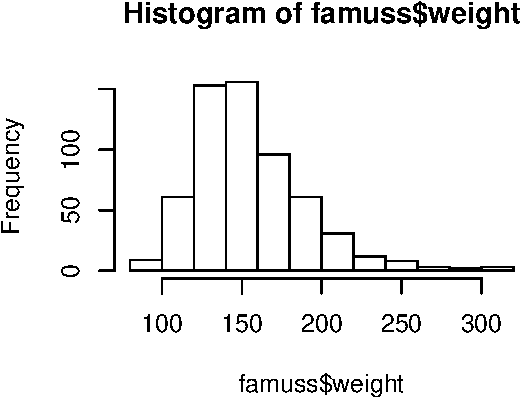
\includegraphics[width=1\linewidth]{001-exploring-data_files/figure-beamer/hist_weight-1} \end{center}

\normalsize

\end{frame}

\begin{frame}{Histograms \dots}
\protect\hypertarget{histograms-1}{}

Histograms show important features of the shape of a distribution:

\begin{itemize}
\item
  Symmetry, or lack of it (skew)
\item
  Minimum and maximum values
\item
  Regions of high frequency (modes)
\end{itemize}

Histograms not so good for:

\begin{itemize}
\item
  Displaying median, quartiles
\item
  Showing subtle skewing
\item
  Identifying extreme values
\end{itemize}

\end{frame}

\begin{frame}{\emph{OI Biostat}, Figure 1.20, frog data}
\protect\hypertarget{oi-biostat-figure-1.20-frog-data}{}

\begin{figure}
\centering
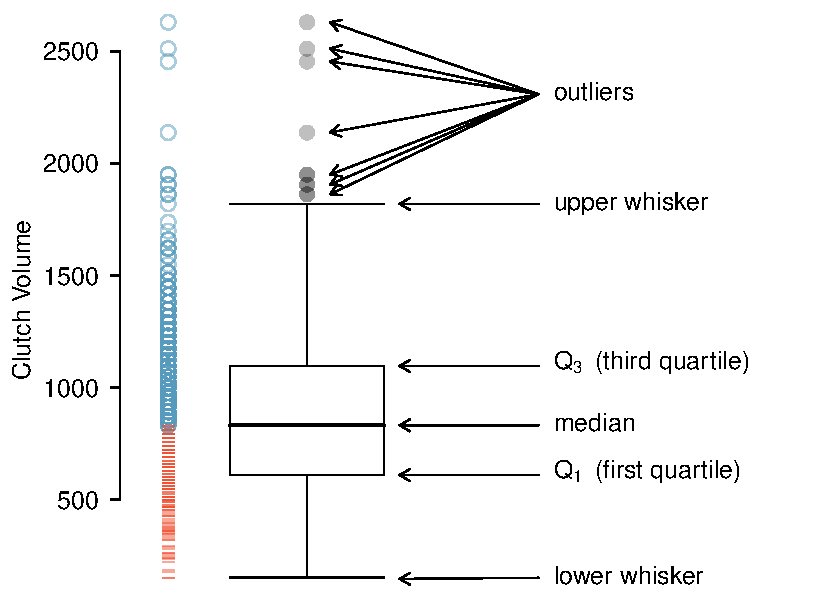
\includegraphics{figures/frogBoxPlot.pdf}
\caption{alt clutch-volume}
\end{figure}

\end{frame}

\begin{frame}{Boxplots}
\protect\hypertarget{boxplots}{}

A boxplot indicates the positions of the first, second, and third
quartiles of a distribution in addition to potential \textbf{outliers},
observations that are far from the center of a distribution.

\begin{itemize}
\item
  Large outliers: values \textgreater{} \(Q_3 + (1.5\times IQR)\)
\item
  Small outliers: values \textless{} \(Q_1 - (1.5 \times IQR)\)
\end{itemize}

On a boxplot\ldots{}

\begin{itemize}
\item
  The rectangle extends from the first quartile to the third quartile,
  with a line at the second quartile (median).
\item
  Whiskers capture data between \(Q_1 - (1.5 \times IQR)\) and
  \(Q_3 + (1.5\times IQR)\) ; whiskers must end at data points.
\item
  Potential outliers shown with dots.
\end{itemize}

\end{frame}

\hypertarget{categorical-data}{%
\section{Categorical data}\label{categorical-data}}

\begin{frame}[fragile]{Tables}
\protect\hypertarget{tables}{}

A table for a single variable, a \emph{frequency table} or \emph{one-way
table}, summarizes the distribution of observations among categories.

Based on the table, describe the distribution of genotype at the
location \emph{actn3.r577x} among the study participants.

\small

\scriptsize

\begin{Shaded}
\begin{Highlighting}[]
\KeywordTok{table}\NormalTok{(famuss}\OperatorTok{$}\NormalTok{actn3.r577x)}
\end{Highlighting}
\end{Shaded}

\begin{verbatim}
## 
##  CC  CT  TT 
## 173 261 161
\end{verbatim}

\normalsize

\end{frame}

\begin{frame}[fragile]{Bar plots for categorical data}
\protect\hypertarget{bar-plots-for-categorical-data}{}

A bar plot is a common way to display a single categorical variable.

\small

\scriptsize

\begin{Shaded}
\begin{Highlighting}[]
\KeywordTok{barplot}\NormalTok{(}\KeywordTok{table}\NormalTok{(famuss}\OperatorTok{$}\NormalTok{actn3.r577x))}
\end{Highlighting}
\end{Shaded}

\begin{center}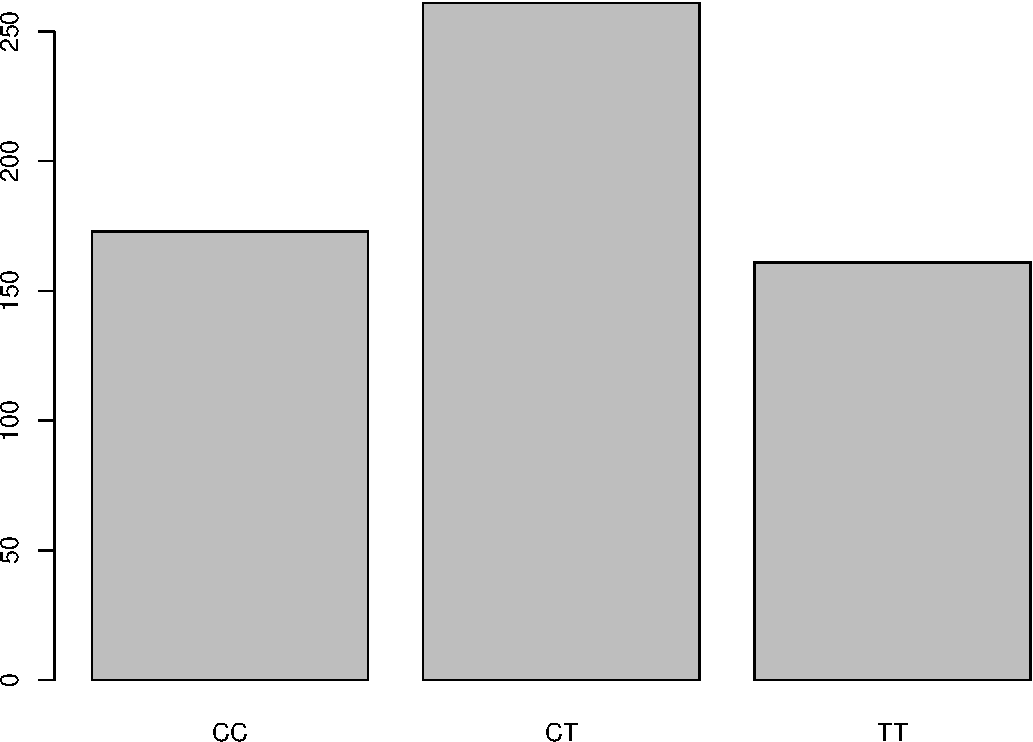
\includegraphics[width=1\linewidth]{001-exploring-data_files/figure-beamer/unnamed-chunk-8-1} \end{center}

\normalsize

\end{frame}

\hypertarget{relationships-between-two-variables}{%
\section{Relationships between two
variables}\label{relationships-between-two-variables}}

\begin{frame}{Summarizing relationships between two variables}
\protect\hypertarget{summarizing-relationships-between-two-variables}{}

Approaches for summarizing relationships between two variables vary
depending on variable types\ldots{}

\begin{itemize}
\item
  Two numerical variables
\item
  Two categorical variables
\item
  One numerical variable and one categorical variable
\end{itemize}

\end{frame}

\begin{frame}{Two numerical variables}
\protect\hypertarget{two-numerical-variables}{}

Two variables \(x\) and \(y\) are

\begin{itemize}
\item
  \emph{positively associated} if \(y\) increases as \(x\) increases.
\item
  \emph{negatively associated} if \(y\) decreases as \(x\) increases.
\end{itemize}

Height and weight are positively associated.

\end{frame}

\begin{frame}[fragile]{Two numerical variables \dots}
\protect\hypertarget{two-numerical-variables-1}{}

\small

\scriptsize

\begin{Shaded}
\begin{Highlighting}[]
\KeywordTok{plot}\NormalTok{(famuss}\OperatorTok{$}\NormalTok{height, famuss}\OperatorTok{$}\NormalTok{weight,}
     \DataTypeTok{xlab =} \StringTok{"Height (in)"}\NormalTok{, }\DataTypeTok{ylab =} \StringTok{"Weight (lb)"}\NormalTok{, }\DataTypeTok{cex =} \FloatTok{0.8}\NormalTok{)  }
\end{Highlighting}
\end{Shaded}

\begin{center}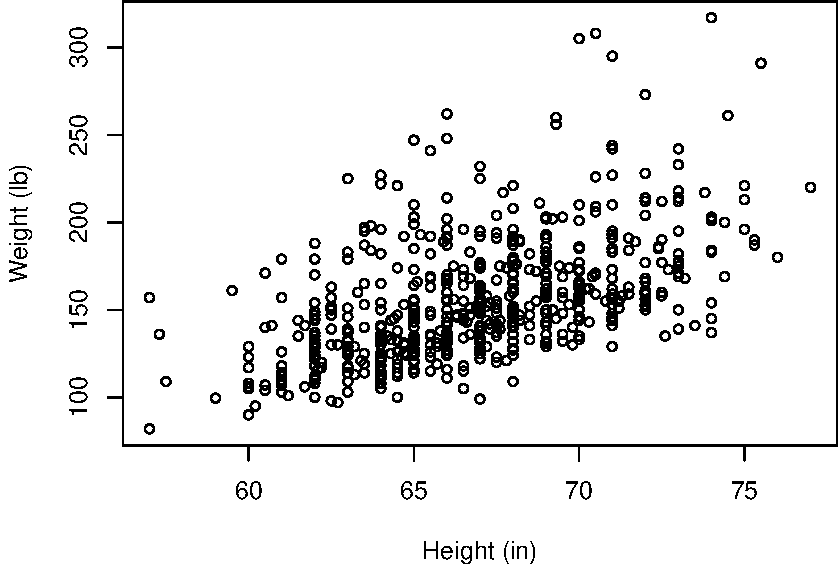
\includegraphics[width=1\linewidth]{001-exploring-data_files/figure-beamer/scatter_height_weight-1} \end{center}

\normalsize

\end{frame}

\begin{frame}[fragile]{Two numerical variables \dots}
\protect\hypertarget{two-numerical-variables-2}{}

Correlation is a numerical summary that measures the strength of a
linear relationship between two variables.

\begin{itemize}
\item
  Introduced in \emph{OI Biostat} Section 1.6.1; details in Ch. 6.
\item
  The correlation coefficient \(r\) takes on values between -1 and 1.
\item
  The closer \(r\) is to \(\pm 1\), the stronger the linear association.
\end{itemize}

\scriptsize

\begin{Shaded}
\begin{Highlighting}[]
\KeywordTok{cor}\NormalTok{(famuss}\OperatorTok{$}\NormalTok{height, famuss}\OperatorTok{$}\NormalTok{weight)}
\end{Highlighting}
\end{Shaded}

\begin{verbatim}
## [1] 0.5308787
\end{verbatim}

\normalsize

\end{frame}

\begin{frame}[fragile]{Two categorical variables}
\protect\hypertarget{two-categorical-variables}{}

A contingency table summarizes data for two categorical variables.

\scriptsize

\begin{Shaded}
\begin{Highlighting}[]
\KeywordTok{addmargins}\NormalTok{(}\KeywordTok{table}\NormalTok{(famuss}\OperatorTok{$}\NormalTok{race, famuss}\OperatorTok{$}\NormalTok{actn3.r577x))}
\end{Highlighting}
\end{Shaded}

\begin{verbatim}
##             
##               CC  CT  TT Sum
##   African Am  16   6   5  27
##   Asian       21  18  16  55
##   Caucasian  125 216 126 467
##   Hispanic     4  10   9  23
##   Other        7  11   5  23
##   Sum        173 261 161 595
\end{verbatim}

\normalsize

\end{frame}

\begin{frame}[fragile]{Two categorical variables \dots}
\protect\hypertarget{two-categorical-variables-1}{}

\scriptsize

\scriptsize

\begin{Shaded}
\begin{Highlighting}[]
\CommentTok{#row proportions}
\KeywordTok{addmargins}\NormalTok{(}\KeywordTok{prop.table}\NormalTok{(}\KeywordTok{table}\NormalTok{(famuss}\OperatorTok{$}\NormalTok{race, famuss}\OperatorTok{$}\NormalTok{actn3.r577x), }\DecValTok{1}\NormalTok{))}
\end{Highlighting}
\end{Shaded}

\begin{verbatim}
##             
##                     CC        CT        TT       Sum
##   African Am 0.5925926 0.2222222 0.1851852 1.0000000
##   Asian      0.3818182 0.3272727 0.2909091 1.0000000
##   Caucasian  0.2676660 0.4625268 0.2698073 1.0000000
##   Hispanic   0.1739130 0.4347826 0.3913043 1.0000000
##   Other      0.3043478 0.4782609 0.2173913 1.0000000
##   Sum        1.7203376 1.9250652 1.3545972 5.0000000
\end{verbatim}

\begin{Shaded}
\begin{Highlighting}[]
\CommentTok{#column proportions}
\KeywordTok{addmargins}\NormalTok{(}\KeywordTok{prop.table}\NormalTok{(}\KeywordTok{table}\NormalTok{(famuss}\OperatorTok{$}\NormalTok{race, famuss}\OperatorTok{$}\NormalTok{actn3.r577x), }\DecValTok{2}\NormalTok{))}
\end{Highlighting}
\end{Shaded}

\begin{verbatim}
##             
##                      CC         CT         TT        Sum
##   African Am 0.09248555 0.02298851 0.03105590 0.14652996
##   Asian      0.12138728 0.06896552 0.09937888 0.28973168
##   Caucasian  0.72254335 0.82758621 0.78260870 2.33273826
##   Hispanic   0.02312139 0.03831418 0.05590062 0.11733618
##   Other      0.04046243 0.04214559 0.03105590 0.11366392
##   Sum        1.00000000 1.00000000 1.00000000 3.00000000
\end{verbatim}

\normalsize

\end{frame}

\begin{frame}{Two categorical variables \dots}
\protect\hypertarget{two-categorical-variables-2}{}

\begin{figure}
\centering
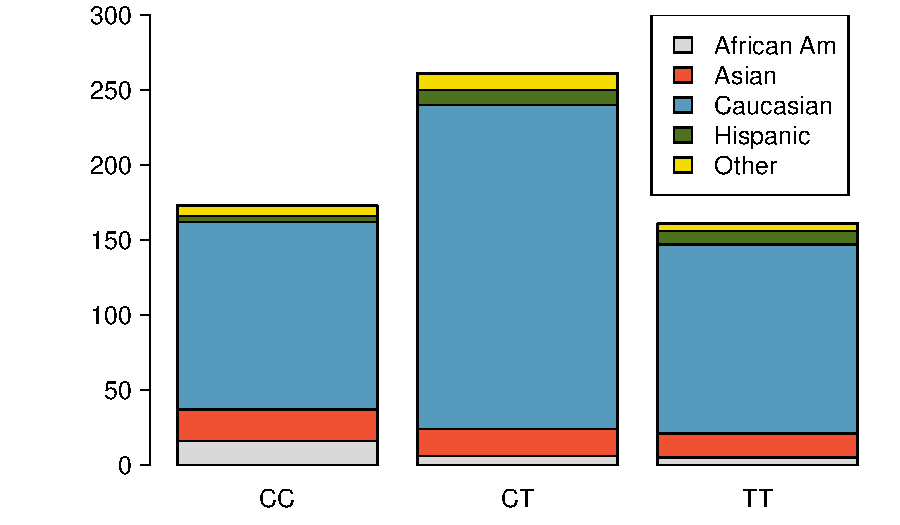
\includegraphics{figures/famussSegBarA.pdf}
\caption{alt text}
\end{figure}

\emph{OI Biostat} Figure 1.35a, segmented bar plot

\end{frame}

\begin{frame}{Two categorical variables \dots}
\protect\hypertarget{two-categorical-variables-3}{}

\begin{figure}
\centering
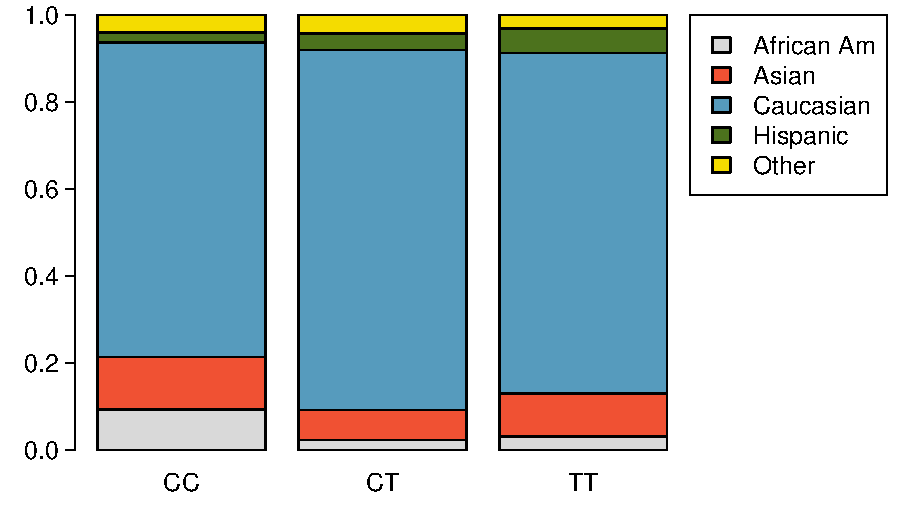
\includegraphics{figures/famussSegBarStaA.pdf}
\caption{standardized segmented barplots}
\end{figure}

\emph{OI Biostat} Figure 1.35b, standardized segmented bar plot

\end{frame}

\begin{frame}{Two categorical variables \dots}
\protect\hypertarget{two-categorical-variables-4}{}

\emph{Relative risk} (RR) is one way of summarizing data presented in a
two-way table of study outcome by participant group.

More in Lab 1 \dots

\end{frame}

\begin{frame}{A numerical variable and a categorical variable}
\protect\hypertarget{a-numerical-variable-and-a-categorical-variable}{}

\emph{FAMuSS} was designed to study the relationship between genotype at
the location \emph{r577x} in the gene \emph{ACTN3} and muscle strength.

Muscle strength was assessed by the percent change in non-dominant arm
strength after resistance training (\texttt{ndrm.ch}).

What visualization would be a good choice to make this comparison?

\end{frame}

\begin{frame}[fragile]{A numerical variable and a categorical variable
\dots}
\protect\hypertarget{a-numerical-variable-and-a-categorical-variable-1}{}

\scriptsize

\scriptsize

\begin{Shaded}
\begin{Highlighting}[]
\KeywordTok{boxplot}\NormalTok{(famuss}\OperatorTok{$}\NormalTok{ndrm.ch }\OperatorTok{~}\StringTok{ }\NormalTok{famuss}\OperatorTok{$}\NormalTok{actn3.r577x)}
\end{Highlighting}
\end{Shaded}

\begin{center}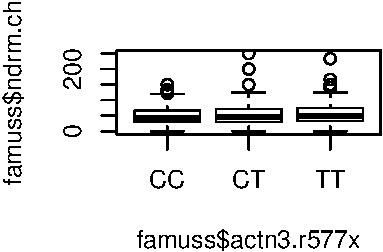
\includegraphics[width=1\linewidth]{001-exploring-data_files/figure-beamer/ndrmbox-1} \end{center}

\normalsize

\end{frame}

\hypertarget{case-study-molecular-cancer-classification}{%
\section{Case study: molecular cancer
classification}\label{case-study-molecular-cancer-classification}}

\begin{frame}{The potential value of genomic data in cancer}
\protect\hypertarget{the-potential-value-of-genomic-data-in-cancer}{}

The majority of cancers are diagnosed by an expert pathologist examining
slides of malignant cells.

Can that be done more accurately by characterizing the genetic makeup of
the malignancy?

\begin{itemize}
\tightlist
\item
  This is perhaps the major potential of genomic characterizations of
  tumors.
\end{itemize}

There are many forms of childhood leukemia.

\begin{itemize}
\item
  Acute myeloblastic leukemia (AML) and acute lymphoblastic leukemia
  (ALL) are the most common.
\item
  AML is a cancer of the bone marrow, where white blood cells
  (lymphocytes) are produced.
\item
  ALL is a cancer of the lymphocytes and is designated as B-cell (ALLB)
  or T-cell (ALLT).
\end{itemize}

\end{frame}

\begin{frame}{Prognosis of the two cancers}
\protect\hypertarget{prognosis-of-the-two-cancers}{}

The probability that a child diagnosed with ALL is survives at least 5
years after the diagnosis is approximately 90\%.

Approximately 65\% of children diagnosed with AML survive at least 5
years.

The diagnosis of leukemia type determines the therapy that will be given
to the child, and the successful treatments for ALL and AML are
different.

In 1999, Todd Golub from the Dana-Farber and the Broad Institute
examined the possibility of classifying leukemia through using a genetic
analysis of a blood sample.

\end{frame}

\begin{frame}{Analyzing the Golub data}
\protect\hypertarget{analyzing-the-golub-data}{}

We can re-analyze the Golub data using tools from graphical and
numerical summaries.

Our analysis will not be identical to the Golub analysis, but will be
similar in spirit.

The tools are straighforward\ldots   

\begin{itemize}
\item
  Thinking through the problem and assembling the tools is the hard
  part.
\item
  The process is more important than the final recipe.
\end{itemize}

\end{frame}

\begin{frame}{Gene expression (details in \emph{OI Biostat})}
\protect\hypertarget{gene-expression-details-in-oi-biostat}{}

\small

\begin{itemize}
\item
  The genetic code stored in DNA contains the information for producing
  the proteins that determine an organism's phenotype.
\item
  Genes that are transcriptionally active (i.e.~turned ``on'') are
  transcribed into messenger RNA (mRNA) that gets translated into
  proteins.
\item
  Genes can be switched on or off, and expressed at varying levels.
  Variations in gene expression produce the range of physical,
  biochemical, and developmental differences in cells and tissues.
\item
  Quantifying the amount of RNA produced in a cell allows for a measure
  of gene expression.
\item
  The transcriptome, or expression profile, is the complete set of RNA
  transcripts produced by the genome in a cell or set of cells.
\end{itemize}

\end{frame}

\begin{frame}{Microarrays (details in \emph{OI Biostat})}
\protect\hypertarget{microarrays-details-in-oi-biostat}{}

\small

\begin{itemize}
\item
  Microarray technology is based on hybridization between two DNA
  strands, in which complementary nucleotide sequences specifically pair
  together.
\item
  The mRNA from a sample is converted into complementary-DNA (cDNA),
  labeled with a fluorescent dye, and added to the microarray.
\item
  When cDNA from the sample encounters complementary DNA probes, the two
  strands will hybridize, allowing the cDNA to adhere to specific spots
  on the slide.
\item
  When the chip is illuminated and scanned, the intensity of
  fluorescence detected at each spot corresponds to the amount of bound
  cDNA.
\item
  DNA microarrays do not directly quantify gene expression levels or
  quantity of mRNA present in a sample.
\item
  The fluorescence intensity data only provide a relative measure of
  gene expression, showing which genes on the chip seem to be more or
  less active in relation to each other.
\end{itemize}

\end{frame}

\begin{frame}{Microarrays}
\protect\hypertarget{microarrays}{}

\begin{figure}
\centering
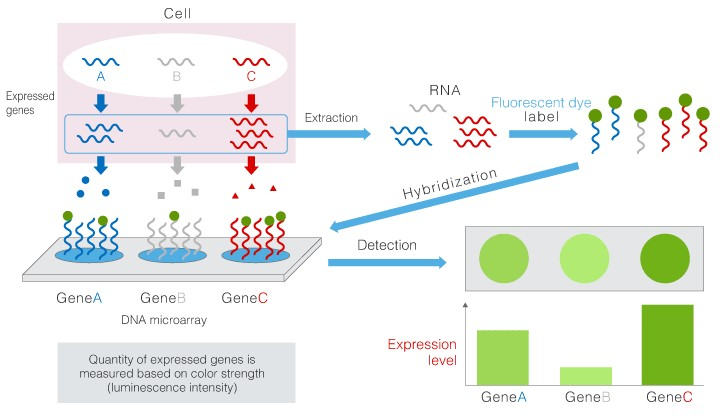
\includegraphics{figures/microarray_schematic.jpg}
\caption{fluorescence detection}
\end{figure}

\end{frame}

\begin{frame}{The Golub clinical data}
\protect\hypertarget{the-golub-clinical-data}{}

Demographic variables described in \emph{OI Biostat} Table 1.54:

\scriptsize

\begin{longtable}[]{@{}ll@{}}
\toprule
\begin{minipage}[b]{0.12\columnwidth}\raggedright
Variable\strut
\end{minipage} & \begin{minipage}[b]{0.82\columnwidth}\raggedright
Description\strut
\end{minipage}\tabularnewline
\midrule
\endhead
\begin{minipage}[t]{0.12\columnwidth}\raggedright
Samples\strut
\end{minipage} & \begin{minipage}[t]{0.82\columnwidth}\raggedright
Sample or chip number. The material from each patient was examined on a
separate chip and experimental run.\strut
\end{minipage}\tabularnewline
\begin{minipage}[t]{0.12\columnwidth}\raggedright
BM.PB\strut
\end{minipage} & \begin{minipage}[t]{0.82\columnwidth}\raggedright
Type of patient material. BM denotes bone marrow; PB denotes a
peripheral blood sample.\strut
\end{minipage}\tabularnewline
\begin{minipage}[t]{0.12\columnwidth}\raggedright
Gender\strut
\end{minipage} & \begin{minipage}[t]{0.82\columnwidth}\raggedright
F for female, M for male.\strut
\end{minipage}\tabularnewline
\begin{minipage}[t]{0.12\columnwidth}\raggedright
Source\strut
\end{minipage} & \begin{minipage}[t]{0.82\columnwidth}\raggedright
Hospital where the patient was treated.\strut
\end{minipage}\tabularnewline
\begin{minipage}[t]{0.12\columnwidth}\raggedright
tissue.mf\strut
\end{minipage} & \begin{minipage}[t]{0.82\columnwidth}\raggedright
A variable showing the combination of type of patient material and sex
of the patient. BM:f denotes bone marrow from a female patient,
etc.\strut
\end{minipage}\tabularnewline
\begin{minipage}[t]{0.12\columnwidth}\raggedright
cancer\strut
\end{minipage} & \begin{minipage}[t]{0.82\columnwidth}\raggedright
The type of leukemia; aml is acute myeloblastic leukemia, allB is acute
lymphoblastic leukemia which started in B-cells (cells that mature into
plasma cells) origin, and allT is acute lymphoblastic leukemia with
T-cell origin (T-cells are a type of white blood cell).\strut
\end{minipage}\tabularnewline
\bottomrule
\end{longtable}

\end{frame}

\begin{frame}{The Golub expression data}
\protect\hypertarget{the-golub-expression-data}{}

The expression data is contained in the last 7,129 columns.

Each column is a variable with a name corresponding to the name of the
probe on the microarray.

The expression levels record fluorescence intensity for each gene.

\begin{itemize}
\item
  The intensity levels have no inherent biological meaning.
\item
  Data have been normalized to adjust for variability between the
  separate arrays used for each patient.
\end{itemize}

\end{frame}

\begin{frame}{Selected variables and columns from Golub data}
\protect\hypertarget{selected-variables-and-columns-from-golub-data}{}

\captionsetup[table]{labelformat=empty}
\scriptsize

\scriptsize

\begin{longtable}[]{@{}rllrrr@{}}
\caption{\emph{OI Biostat} Table 1.40}\tabularnewline
\toprule
Samples & Gender & cancer & AFFX-BioB-5\_at & AFFX-BioB-M\_at &
AFFX-BioB-3\_at\tabularnewline
\midrule
\endfirsthead
\toprule
Samples & Gender & cancer & AFFX-BioB-5\_at & AFFX-BioB-M\_at &
AFFX-BioB-3\_at\tabularnewline
\midrule
\endhead
39 & F & allB & -1363.28 & -1058.59 & -541.47\tabularnewline
40 & F & allB & -796.29 & -1167.10 & 7.54\tabularnewline
42 & F & allB & -679.14 & -1069.83 & -690.30\tabularnewline
47 & M & allB & -1164.40 & -1109.94 & -990.13\tabularnewline
48 & F & allB & -1299.65 & -1402.00 & -1077.54\tabularnewline
\bottomrule
\end{longtable}

\normalsize

\end{frame}

\begin{frame}{Analyzing the Golub leukemia data}
\protect\hypertarget{analyzing-the-golub-leukemia-data}{}

We will do an analysis in class using some of the simple but
surprisingly powerful ideas behind numerical and graphical summaries.

The goal of the Golub study was to develop a procedure for
distinguishing between AML and ALL based only on the gene expression
levels of a patient. There are two major issues to be addressed:

\begin{enumerate}
\item
  Which genes are the most informative for making a prediction?
\item
  What is a workable strategy for predicting leukemia type from
  expression data for a specific set of genes?
\end{enumerate}

\end{frame}

\begin{frame}[fragile]{Starting small\ldots{}}
\protect\hypertarget{starting-small}{}

\footnotesize

\scriptsize

\begin{verbatim}
##    cancer        A         B        C        D
## 69   allB 39307.96 35232.401 41170.76 35792.79
## 67   allT 32281.88 41432.024 59328.51 49608.14
## 55   allB 47429.94 35568.928 56074.96 42857.78
## 56   allB 25533.87 16983.749 28056.75 32693.92
## 59   allB 35960.55 24191.746 27637.90 22240.75
## 52    aml 46177.95  6189.465 12557.24 34485.41
## 53    aml 43790.70 33661.825 38380.30 29758.25
## 51    aml 53420.05 26109.245 31427.20 23809.70
## 50    aml 41241.59 37589.773 47325.77 30099.36
## 54    aml 41300.57 49198.412 66026.10 56248.62
\end{verbatim}

\normalsize

\end{frame}

\end{document}
